% !TEX root =  ../main_manuscript.tex 
\section{Results}
\subsection{Model Results}
In PRIAS, the rate of reclassification within the first five years was 35\%. This rate was capped at a maximum of 50\% in external GAP3 cohorts (Panel~B, Figure~\ref{fig:auc_beforecalib}). That is, many patients do not require any biopsy in the first five years. 

In the fitted joint model, for every ten year increase in patient age (difference between 75-th and 25-th percentile of patient age) the adjusted hazard ratio of reclassification is 1.45~(95\%CI:~1.30--1.63). When fitted PSA value (log scale) increases from 2.36 to 3.07 (25-th to 75-th percentile), the adjusted hazard ratio of reclassification is 0.99~(95\%CI:~0.89--1.11). When estimated instantaneous PSA (log scale) velocity increases from -0.09 to 0.31 (25-th to 75-th percentile), the adjusted hazard ratio is 2.47~(95\%CI:~1.93--2.99). Hence, instantaneous velocity of PSA (log scale) is a stronger predictor for reclassification than its value. Detailed parameter estimates are in Supplementary~A.2.

\subsection{Validation Results}
The time-varying AUC and calibration of our model in different cohorts is shown in Panel~A and Panel~B of Figure~\ref{fig:auc_beforecalib}, respectively. The AUC achieves a moderate level in all cohorts. It fluctuates roughly around 0.63 over time. In terms of calibration, our model seems well calibrated only for the Johns Hopkins AS cohort. However, this issue was resolved (Figure~6, Supplementary~B) upon recalibration of our model's baseline hazard of reclassification separately for each cohort. We found trivial differences in risk predictions for individual patients from our recalibrated joint model, and from separately fitted new joint models for each cohort (Figure~7, Supplementary~B). Comprehensive discussion of validation results is in Supplementary~B.

\begin{figure}
\centerline{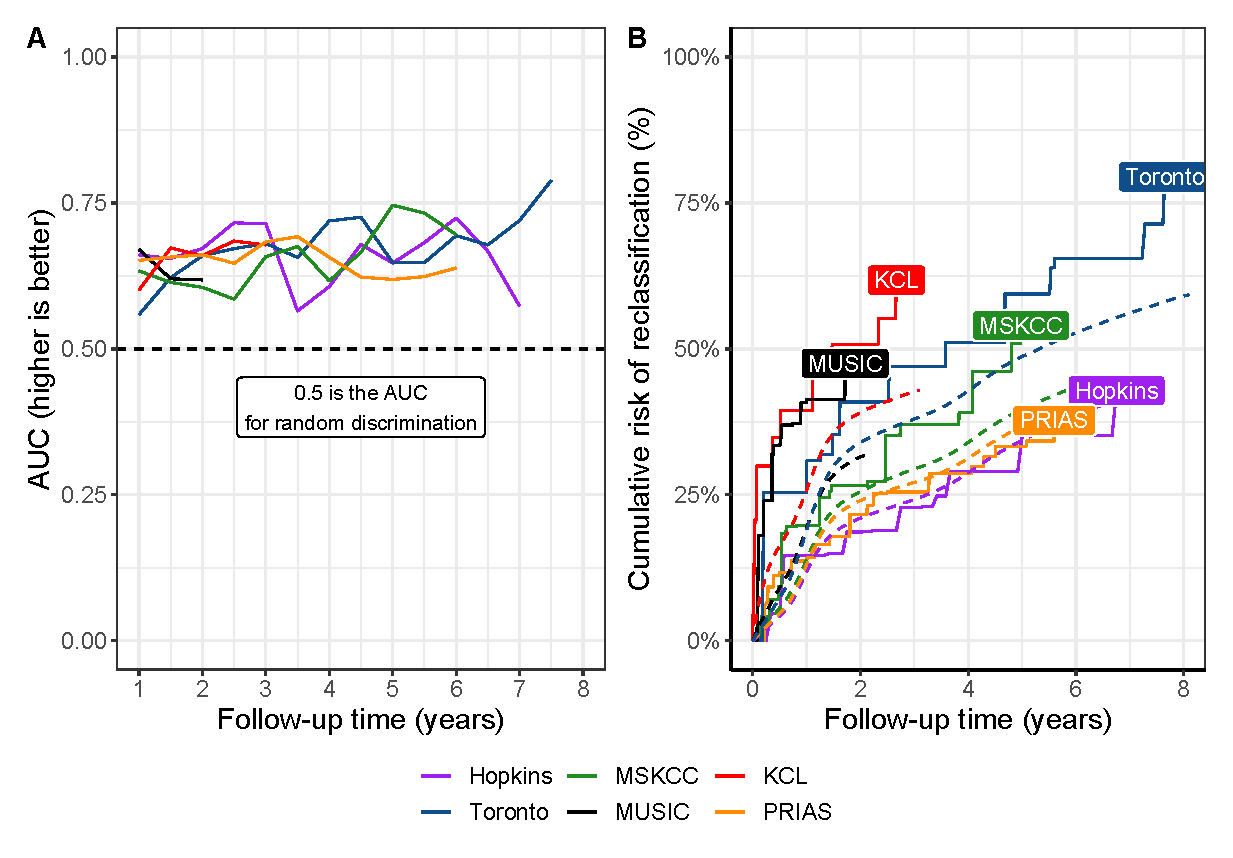
\includegraphics[width=\columnwidth]{images/auc_beforecalib.eps}}
\caption{\textbf{Model Validation Results}. \textbf{Panel~A}: time dependent area under the receiver operating characteristic curve or AUC (measure of discrimination). \textbf{Panel~B}: calibration-at-large~\citep{royston2013external,steyerberg2010assessing}, with solid lines depicting the non-parameteric estimate of the cumulative-risk of reclassification~\citep{turnbull1976empirical}, and dashed lines showing the average cumulative-risk of reclassification obtained using the joint model fitted to the PRIAS dataset. Full names of Cohorts are \textit{PRIAS}: Prostate Cancer International Active Surveillance, \textit{Toronto}: University of Toronto Active Surveillance, \textit{Hopkins}: Johns Hopkins Active Surveillance, \textit{MSKCC}: Memorial Sloan Kettering Cancer Center Active Surveillance, \textit{KCL}: King's College London Active Surveillance, \textit{MUSIC}: Michigan Urological Surgery Improvement Collaborative Active Surveillance.}
\label{fig:auc_beforecalib}
\end{figure}

\subsection{Personalized Schedule Results}
Various personalized and fixed biopsy schedules for demo patients are shown in Figure \ref{fig:demo_pat1} 

In addition, we scheduled biopsies only for the first ten years follow-up because of limited follow-up period of the training dataset PRIAS. A compulsory biopsy was done scheduled year ten of follow-up in all schedules for meaningful comparison of their expected delays in detection of GS7. and Appendix C's Figure 6, 7, 8 and 9. The biopsies denoted by `B' show that personalized schedules schedule fewer biopsies than fixed schedules. At the same time the expected time delay in detection of GS7 is less than an year for personalized schedules. We have implemented this approach in a web-application (\url{https://emcbiostatistics.shinyapps.io/prias_biopsy_recommender/}, and Appendix D) for practical use.